%%%%%%%%%%%%%%%%%%%%%%%%%%%%%%%%%%%%%%%%%%%%%%%%%%%%%%%%%%%%%%%%%%%%%%%%%%%%%%
% Short Sectioned Assignment LaTeX Template Version 1.0 (5/5/12)
% This template has been downloaded from: http://www.LaTeXTemplates.com
% Original author: Frits Wenneker (http://www.howtotex.com)
% License: CC BY-NC-SA 3.0 (http://creativecommons.org/licenses/by-nc-sa/3.0/)
%%%%%%%%%%%%%%%%%%%%%%%%%%%%%%%%%%%%%%%%%%%%%%%%%%%%%%%%%%%%%%%%%%%%%%%%%%%%%%

\documentclass[11pt, a4paper]{book}

% Desactiva la distribución vertical automática
\raggedbottom

% PAQUETES ------------------------------------------------------------------------------

\usepackage[T1]{fontenc}
\usepackage[utf8]{inputenc}
% Selecciona el español para palabras introducidas automáticamente, p.ej. "septiembre" en la fecha y especifica que se use la palabra Tabla en vez de Cuadro
\usepackage[spanish,es-tabla,es-nodecimaldot]{babel}
\usepackage{amsmath}
\usepackage{amsfonts}
\usepackage{amssymb}
% Manejo de símbolos de cita múltiples
\usepackage{csquotes}
% Figuras e imágenes
\usepackage{graphics, graphicx, float}
% Permite dar estilo a los subtítulos de las figuras (leyendas)
\usepackage{caption}
% Permite sub-leyendas en sub-figuras (figuras dentro de figuras)
\usepackage{subcaption}
% Permite múltiples filas en tablas
\usepackage{multirow}
% Elimina numeración de paginas en blanco
\usepackage{emptypage}
% Añade más funcionalidades a las listas
\usepackage{enumitem}
% Introduce la bibliografía en el índice
\usepackage[nottoc]{tocbibind}
% Permite continuar con la numeración entre listas distintas
% \usepackage{fourier} % Use the Adobe Utopia font for the document
\usepackage{url} % ,href} %para incluir URLs e hipervínculos dentro del texto (aunque hay que instalar href)
% Para incluir el símbolo del euro
\usepackage[gen]{eurosym} 
\usepackage{cite} %para incluir citas del archivo <nombre>.bib
% \usepackage{enumerate}
% Permite añadir comentarios multilínea que no se mostrarán en el PDF final
\usepackage{comment}
\usepackage{tabularx}
\usepackage{booktabs}
\usepackage[table,xcdraw]{xcolor}
% Marca en rojo los elementos pendientes (TO-DOs)
\newcommand{\todo}[1]{\textcolor{orange}{TODO: #1}}
% Permite que el contador de footnotes no se reinicie en cada capítulo
\usepackage{chngcntr}
\counterwithout{footnote}{chapter}
% Diagramas de Gantt
\usepackage{tikz}
\usepackage{pgfgantt}
% Formato apaisado
\usepackage{pdflscape}
% Permite crear tablas largas que se dividen en varias páginas
\usepackage{longtable}
% Permite crear tablas con celdas de ancho variable
\usepackage{array}
% Para el pseudo-código
\usepackage{algorithm}
\usepackage{algpseudocode}

% ESTILOS DE PAGINA ------------------------------------------------------------------
\renewcommand{\familydefault}{\sfdefault}
% Modificar encabezamientos y pie de páginas
\usepackage{fancyhdr}
\pagestyle{fancyplain} % Makes all pages in the document conform to the custom headers and footers
\fancyhead[L]{} % Empty left header
\fancyhead[C]{} % Empty center header
% \fancyhead[R]{Francisco David Castejón Soto} % Nombre del autor en el encabezado derecho
\fancyfoot[L]{} % Empty left footer
\fancyfoot[C]{} % Empty center footer
\fancyfoot[R]{\thepage} % Page numbering for right footer
\renewcommand{\headrulewidth}{0pt} % Remove header underlines
\renewcommand{\footrulewidth}{0pt} % Remove footer underlines
\setlength{\headheight}{13.6pt} % Customize the height of the header

\usepackage{titlesec, blindtext, color}
\definecolor{gray75}{gray}{0.75}
\newcommand{\hsp}{\hspace{20pt}}
\titleformat{\chapter}[hang]{\Huge\bfseries}{\thechapter\hsp\textcolor{gray75}{|}\hsp}{0pt}{\Huge\bfseries}
\setcounter{secnumdepth}{4}
\usepackage[Lenny]{fncychap}

% For code snippets
\usepackage{minted}
\usemintedstyle{colorful}
% Control de enlaces hipertexto en el documento. Este paquete debe cargarse el último.
\usepackage{hyperref}
\hypersetup{
	colorlinks=true,	% false: boxed links; true: colored links
	linkcolor=black,	% color of internal links
	urlcolor=cyan		% color of external links
}

% Información del documento ---------------------------------------------------------
\author{Francisco David Castejón Soto}
\title{Desarrollo y Optimización de un Agente Inteligente para Scripts of Tribute mediante Algoritmos Evolutivos}
\date{\today}

% DOCUMENTO -------------------------------------------------------------------------
\begin{document}

% Páginas preliminares sin numeración
\frontmatter

\begin{titlepage}
	\thispagestyle{empty}

	\centering
	\includegraphics[width=0.9\textwidth]{logos/logo_ugr.jpg}
	\vspace{1.0cm}

	{\rmfamily\textsc{\Large MÁSTER UNIVERSITARIO}}\\[0.2cm]
	{\rmfamily\textsc{\large en Ciencia de Datos e Ingeniería de Computadores}}
	\vspace{1.5cm}

	\vfill

	{\Huge\bfseries Trabajo de Fin de Máster}\\[0.5cm]
	\rule{\textwidth}{2pt}\\[0.5cm]
	{\Large\bfseries Desarrollo y Optimización de un Agente Inteligente \\
	para Scripts of Tribute mediante Algoritmos Evolutivos}
	\vspace{1.5cm}

	\vfill

	\begin{tabular}{@{}c@{}}
		\textbf{\large Autor}         \\[0.3cm]
		Francisco David Castejón Soto \\[1cm]
		\textbf{\large Director}      \\[0.3cm]
		Dr. Pablo García Sánchez
	\end{tabular}

	\vfill

	\includegraphics[width=0.4\textwidth]{logos/etsiit_logo.png}\\[0.3cm]
	{\rmfamily\textsc{\footnotesize Escuela Técnica Superior de Ingenierías Informática y de Telecomunicación}}\\
	\rule{0.1\textwidth}{0.5pt}\\[0.3cm]
	{\large Granada, 1 Julio de 2025}

\end{titlepage}
\chapter*{Prefacio}

Para la realización de este documento, se ha utilizado la plantilla \LaTeX \cite{guervos_jjplantilla-tfg-etsiit_2024} específica para la ETSIIT.
\chapter*{Agradecimientos} \label{ch:agradecimientos}

A mi familia por el apoyo que me han brindado incondicionalmente durante estos años fuera de casa. Y a mi pareja, por mostrarme más caminos de los que nunca hubiera pensado que existieran para mí.
\chapter*{Resumen}

{\large\textbf{Resumen}}

En el ámbito de la inteligencia artificial para videojuegos, la creación de agentes autónomos que actúen como jugadores virtuales sigue siendo un desafío considerable. Este trabajo aborda dicho desafío en el contexto del motor de simulación \textit{Scripts of Tribute} para el juego de cartas \textit{Tales of Tribute}, presentando el diseño y la implementación de un sistema completo para el entrenamiento de un bot competitivo mediante técnicas evolutivas.

La metodología se articula en dos componentes principales. Primero, se desarrolló un agente cuya toma de decisiones se basa en una función de evaluación heurística, parametrizada por un vector de pesos que pondera distintas facetas del estado del juego. Segundo, se construyó un sistema de entrenamiento que utiliza un algoritmo de estrategia evolutiva, para optimizar dicho vector de pesos. Para ello, se implementaron y compararon diversas arquitecturas de evaluación, incluyendo un modo fijo contra oponentes estáticos, un modo de coevolución para fomentar la competición interna, y un modo híbrido que combina ambas estrategias. Adicionalmente, se integró un mecanismo de ``salón de la fama'' para preservar a los individuos de élite y combatir el olvido catastrófico.

Los resultados experimentales demuestran una clara especialización de los agentes en función del modo de entrenamiento. Además, el salón de la fama implementado es beneficioso en función de la estabilidad del objetivo de la población. En última instancia, se concluye que el sistema propuesto es capaz de generar agentes competitivos, validando la eficacia del enfoque evolutivo para la optimización de la toma de decisiones en juegos de estrategia.

\vspace{\baselineskip}
\noindent\textbf{Palabras clave:} Inteligencia Artificial para Videojuegos, Algoritmos Evolutivos, Estrategias Evolutivas, Coevolución, Juegos de Cartas.

\newpage
{\large\textbf{Abstract}}

\vspace{0.5\baselineskip}

\textit{In the field of artificial intelligence for video games, the creation of autonomous agents that act as virtual players remains a considerable challenge. This report addresses that challenge in the context of the simulation engine \textit{Scripts of Tribute} for the card game \textit{Tales of Tribute}, presenting the design and implementation of a complete system for training a competitive bot using evolutionary techniques.}

\textit{The methodology is articulated in two main components. First, an agent was developed whose decision making is based on a heuristic evaluation function, parameterized by a vector of weights that weights different facets of the game state. Second, a training system using an evolutionary strategy algorithm was built to optimize this vector of weights. For this purpose, several evaluation architectures were implemented and compared, including a fixed mode against static opponents, a co-evolution mode to encourage internal competition, and a hybrid mode combining both strategies. Additionally, a ``hall of fame'' mechanism was integrated to preserve elite individuals and combat catastrophic forgetting.}

\textit{The experimental results demonstrate a clear specialization of the agents as a function of the training mode. Moreover, the implemented hall of fame is beneficial as a function of the stability of the population objective. Ultimately, it is concluded that the proposed system is able to generate competitive agents, validating the effectiveness of the evolutionary approach for the optimization of decision making in strategy games.}

\vspace{\baselineskip}
\noindent\textbf{Keywords:} Artificial Intelligence for Video Games, Evolutionary Algorithms, Evolution Strategies, Coevolution, Card Games.

% Índices
\cleardoublepage
\tableofcontents

\cleardoublepage
\listoffigures

\cleardoublepage
\listoftables

% Contenido principal
\mainmatter

\part{Marco teórico} \label{part:idea}
\chapter{Introducción} \label{chap:introduccion}

% Hablar la importancia de la IA en los videojuegos, especialmente en los de estrategia
% Introducir brevemente el concepto de algoritmos evolutivos como técnica para entrenar agentes
% Concluir presentando el problema que se aborda: entrenar un bot para el juego "Tales of Tribute"

La inteligencia artificial (IA) en videojuegos existe en una intersección entre la ciencia computacional y el arte del entretenimiento, dando vida a mundos virtuales y creando oponentes dignos de nuestras mejores estrategias. En este contexto, la IA se refiere únicamente a un conjunto de algoritmos y técnicas diseñadas para cumplir una función muy específica dentro del videojuego. Ejemplos de esto son la IA que ``conduce'' los coches en un juego de carreras, los Pokémon contra los que el jugador se enfrenta en una batalla o el simple movimiento de una línea de píxeles (a modo de pala contrincante) en el videojuego Pong. Esta acepción específica contrasta con la idea más extendida de IA, que posee un conjunto de definiciones más amplias y generalistas como ``la máquina que aprende'' o ``el estudio y construcción de sistemas que hacen <<lo correcto>>, en función de su objetivo'' \cite{russell_artificial_2021}.

Independientemente de la definición que se utilice, lo cierto es que un factor clave en el desarrollo de un videojuego es la creación de una IA que resulte entretenida para el jugador. De la misma forma que en un libro o una película es necesaria una trama que plantee un desafío, como la lucha contra el Imperio Galáctico en Star Wars, o un compañero de aventuras que ayude al protagonista, como Sam en El Señor de los Anillos, en un videojuego es necesaria una IA que controle esos elementos que interactúan con el jugador, ya sean enemigos, aliados o incluso el propio entorno. Desde los propios inicios de la industria del videojuego, donde se construían máquinas específicas para ejecutar un juego concreto, como es el caso de Nim en 1948 \cite{redheffer_machine_1948}, hasta los videojuegos modernos, donde se utilizan técnicas de IA más complejas, como el aprendizaje por refuerzo (más en la sección \ref{sec:estado_arte}), la IA ha sido un componente esencial para crear experiencias de juego atractivas y desafiantes.

La intención de este trabajo es la de crear una IA contra la que jugar en un videojuego de estrategia. En concreto, la IA que controla a un agente autónomo (o simplemente ``bot'') en el videojuego de cartas \textit{Tales of Tribute}. Es importante la distinción entre ``juego'' y ``videojuego'' en este caso, ya que las cartas no son físicas, sino que únicamente existen en el universo digital del videojuego. Para guiar las decisiones del bot, un algoritmo evolutivo se encarga de ajustar los pesos que se utilizan para calcular la puntuación de cada jugada posible, eligiendo vorazmente la jugada que maximiza dicha puntuación. Así se ha conseguido crear un contrincante que juega de forma competitiva tanto contra el jugador humano como contra otros bots manejados por IAs totalmente diferentes.
\chapter{Objetivos}


\section{Objetivo principal}


\section{Objetivos generales}


\section{Objetivos específicos}



\chapter{Antecedentes}

\section{Inteligencia artificial en videojuegos}
%% Hablar sobre las técnicas comunes de IA en juegos (máquinas de estados, árboles de comportamiento, MCTS)


\section{Estado del arte}
% Qué técnicas se están usando actualmente

\section{Trabajos relacionados}
% Paper de Pablo y TFG de los ganadores de la competición de IA de Tales of Tribute.
% Comparar sus enfoques al mio
\chapter{Plataforma de trabajo} \label{chap:plataforma_trabajo}

Una vez establecidos los objetivos del proyecto y habiendo explorado el contexto de la inteligencia artificial en la industria del videojuego, es fundamental detallar la plataforma sobre la cual se ha erigido el trabajo práctico. Este capítulo se dedica a describir en profundidad los dos pilares que constituyen el campo de pruebas del agente: el videojuego de cartas \textit{Tales of Tribute} y, de forma más importante, su \textbf{motor de simulación de código abierto}, \textit{Scripts of Tribute}. Para poder comprender las decisiones que se han tomado durante el desarrollo del bot, es necesario conocer primero las reglas del entorno en el que opera. Por ello, se comenzará explicando las reglas y mecánicas del videojuego. Posteriormente, se analizará la arquitectura del entorno de simulación, que no solo hace posible el enfrentamiento entre bots, sino que también ha servido de base para competiciones académicas internacionales.


\section{El videojuego: \textit{Tales of Tribute}} \label{sec:tales_of_tribute}

\textit{Tales of Tribute} es un videojuego de cartas para dos jugadores del género de construcción de mazos, que existe dentro del popular videojuego \textit{The Elder Scrolls Online}. En la figura \ref{fig:tales_tablero} se puede ver una captura del tablero de juego, donde se han numerado los elementos principales para facilitar su identificación \cite{pixel_eso_2022}.

El objetivo principal del juego es conseguir puntos de prestigio\footnote{El prestigio es la métrica principal de victoria en \textit{Tales of Tribute}. Se podría considerar un análogo a los ``puntos de vida'' en otros juegos, pero en este caso, el objetivo es acumularlos en vez de reducir los del oponente.}, el cual se puede consultar en su marcador (elemento 11 en la figura \ref{fig:tales_tablero}). Hay varias formas de ganar: un jugador consigue la victoria si alcanza 40 puntos de prestigio y mantiene la ventaja tras el turno de su oponente. Si no lo consigue, el juego continúa hasta que alguno de los dos jugadores alcance los 80 puntos. Existe, además, una condición de victoria alternativa que se consigue al ganarse el favor de todos los ``patrones'', un tipo de mecánica especial que se detallará más adelante.

\begin{figure}[H]
	\centering
	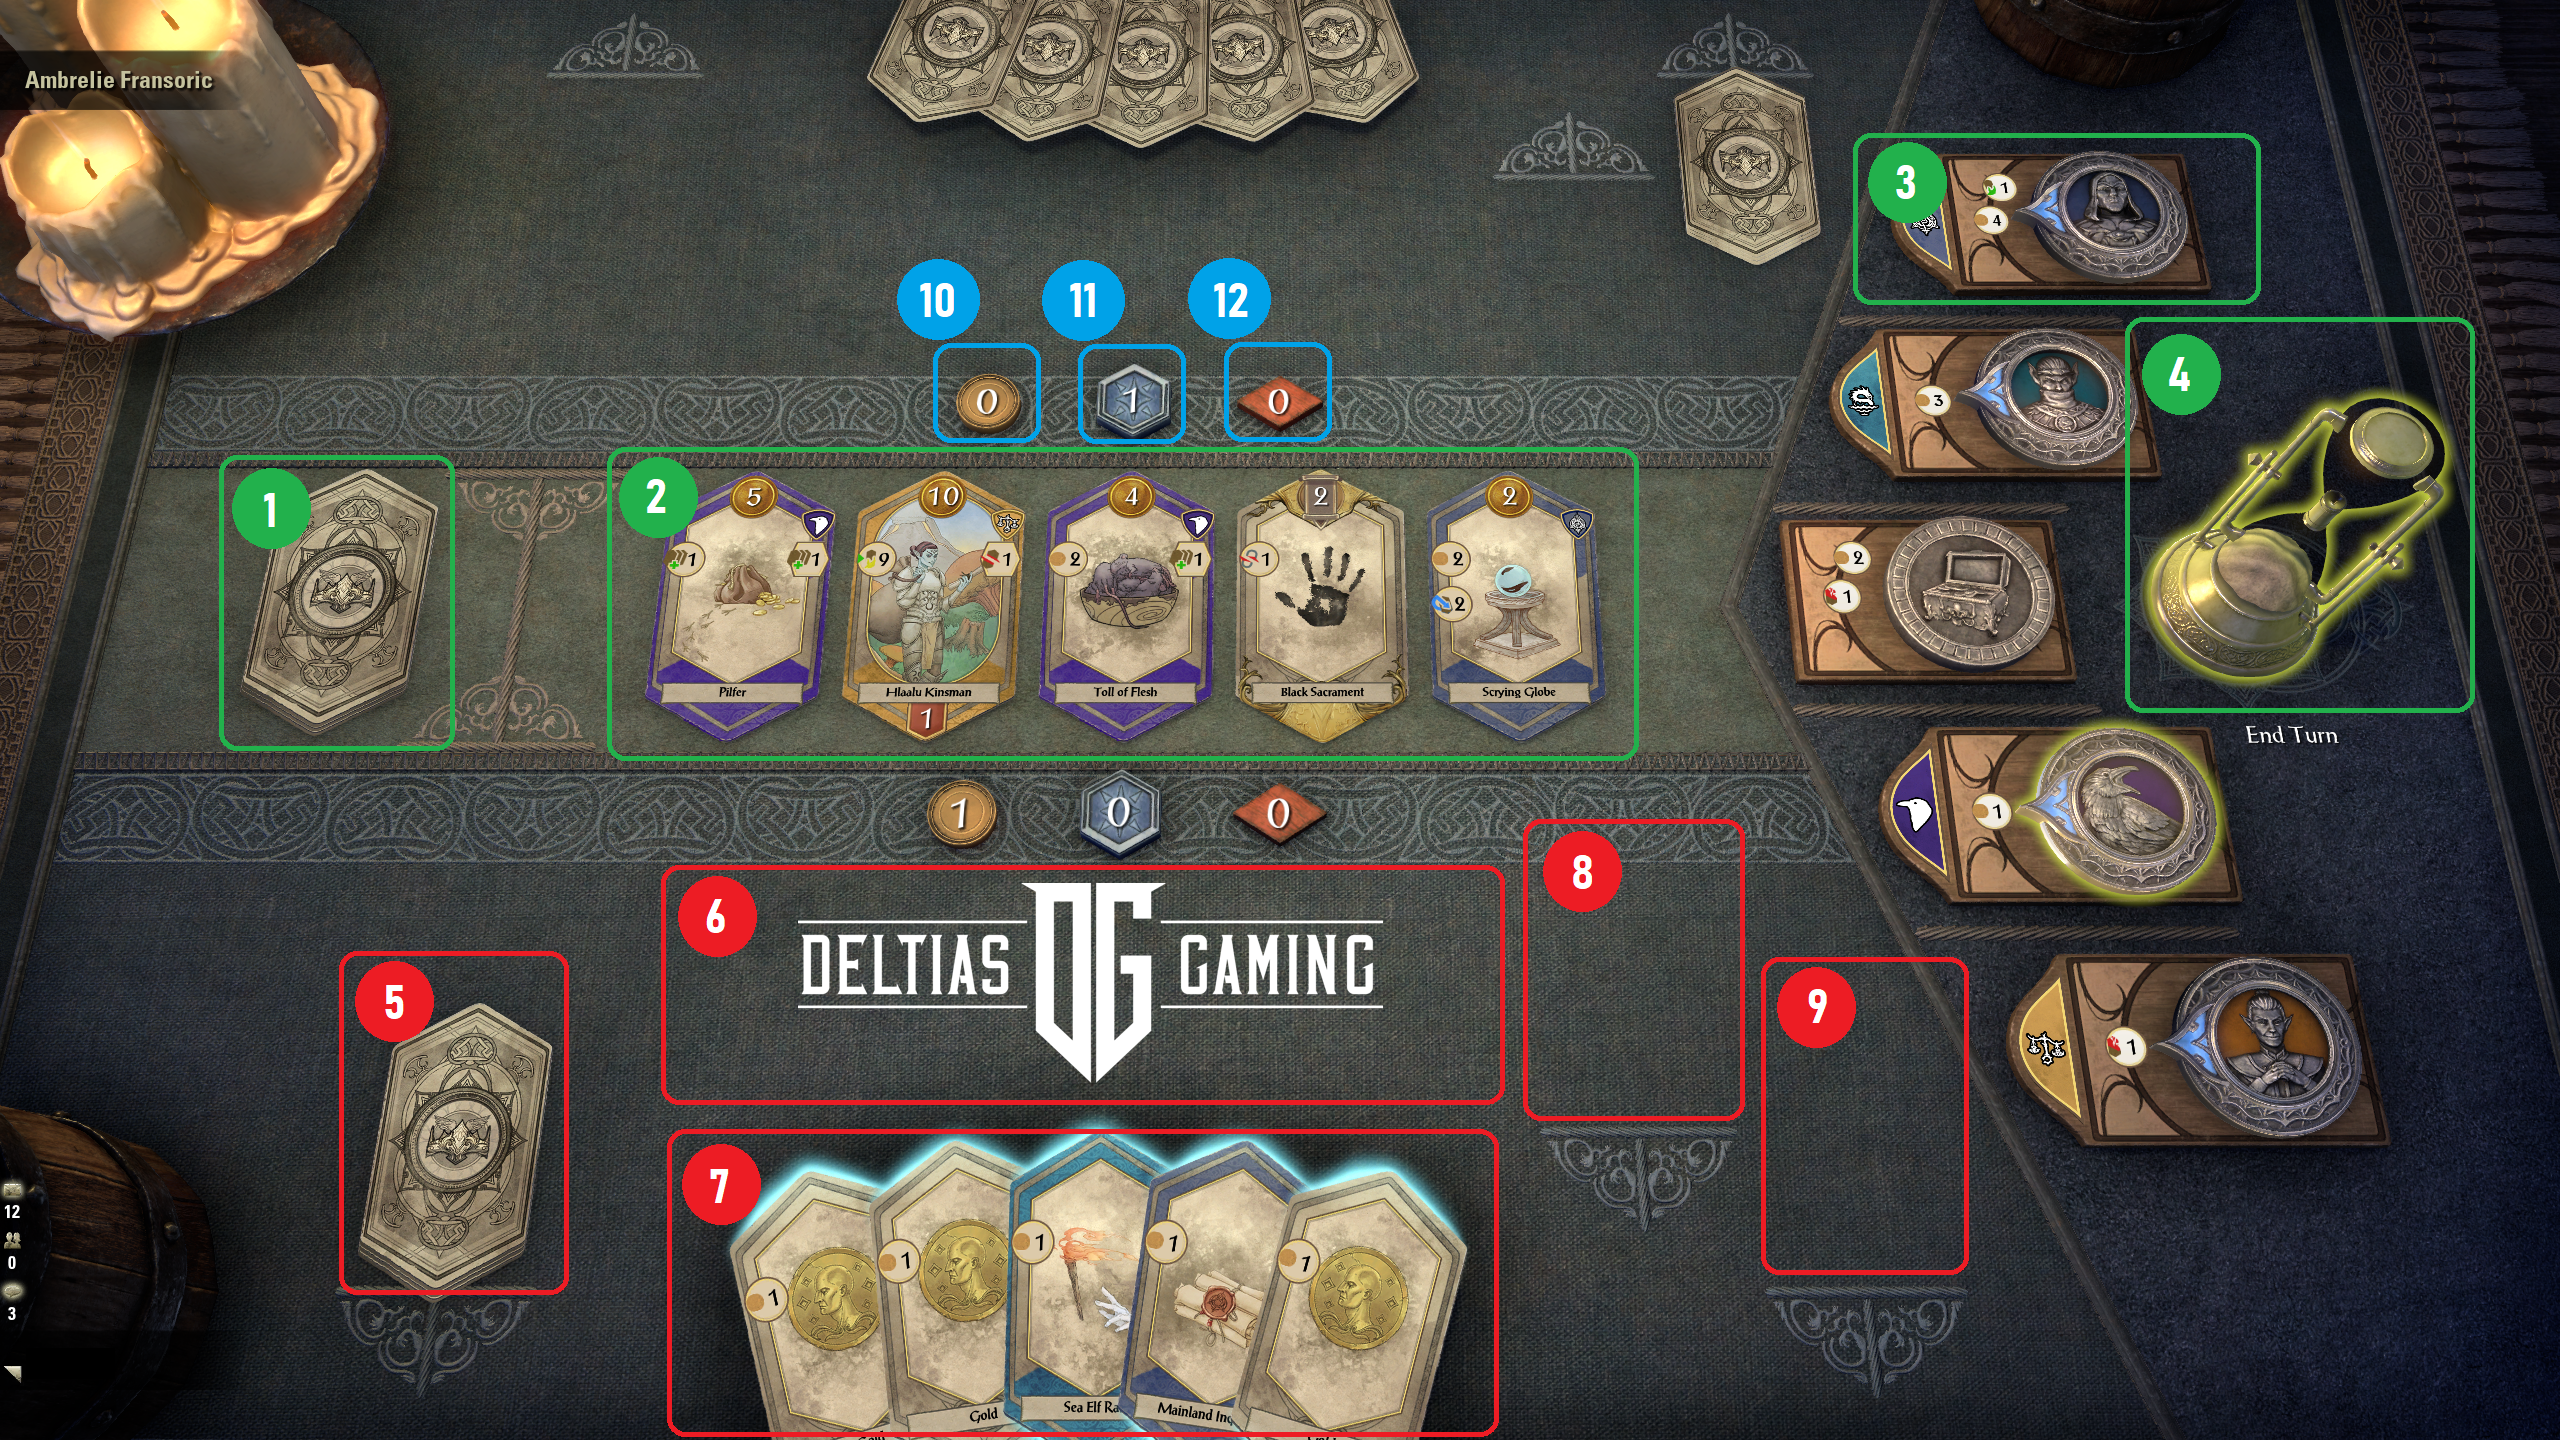
\includegraphics[width=1.0\textwidth]{img/tales_tablero.png}
	\caption{Tablero de juego de Tales of Tribute, con sus componentes principales numerados. \cite{pixel_eso_2022}}
	\label{fig:tales_tablero}
\end{figure}

Al comienzo de cada partida, ambos jugadores deben elegir con qué conjuntos de cartas quieren jugar. Para ello, se presentan siete mazos, cada uno asociado a un patrón (elemento 3), y los jugadores se turnan para seleccionar un total de cuatro. Estos cuatro mazos, junto con un mazo estándar asociado a la ``Tesorería'' que está presente en todas las partidas, se barajan conjuntamente para formar el mazo de robo de la Taberna (elemento 1). De este mazo se revelan cinco cartas en el área de la Taberna (elemento 2), que son las cartas que los jugadores podrán adquirir durante la partida. La esencia de la construcción de mazos reside en que ambos jugadores comienzan con un pequeño mazo de diez cartas básicas idénticas y, a lo largo de la partida, utilizan los recursos que estas generan para comprar cartas más poderosas de la Taberna, añadiéndolas a su propio ciclo de cartas. Además, el jugador que tiene el turno en segundo lugar obtiene una pequeña recompensa de 1 moneda debido a que cuenta con la desventaja de que su oponente ha podido jugar primero.

La estructura de un turno es la siguiente, el jugador activo roba cinco cartas de su mazo personal (elemento 5) para formar su mano (elemento 7). Jugar una carta no tiene coste y, al hacerlo, se activan sus efectos y se mueve a una pila de descarte temporal (elemento 8). Al final del turno, todas las cartas sin jugar aun en la mano y en la pila de descarte temporal se mueven a la pila de reposo (elemento 9). Cuando el mazo de robo personal se agota, la pila de reposo se baraja y se convierte en el nuevo mazo de robo, completando el ciclo. De esta manera, las cartas adquiridas se incorporan progresivamente al mazo del jugador, haciéndolo cada vez más potente.

Las cartas se pueden clasificar en dos tipos principales: acciones y agentes. Las ``cartas de acción'' producen un efecto inmediato (como ganar monedas u obtener puntos de poder) y después se descartan. Por otro lado, las ``cartas de agente'' también tienen un efecto inmediato, pero tras jugarse, se colocan en el tablero en la zona de agentes activos (elemento 6). Estos agentes permanecen en juego y su habilidad puede ser activada una vez por turno, proporcionando una ventaja continua. Sin embargo, el oponente puede destruirlos de diferentes maneras, como utilizando puntos de poder (elemento 12), donde cada punto inflige un punto de daño al agente. Existen, además, las ``cartas de contrato'', que son versiones de un solo uso de las acciones y agentes, siendo eliminadas del juego permanentemente tras su primer uso o al ser derrotadas. Este tipo de cartas de contrato son las que se han utilizado para crear heurísticas específicas en el bot, ya que sus efectos pueden ser muy poderosos.

Finalmente, además de jugar y comprar cartas, los jugadores disponen de otras acciones estratégicas. La más importante es la posibilidad de interactuar con uno de los cuatro patrones elegidos al principio de la partida. Cada patrón ofrece una habilidad única a cambio de un coste en monedas, poder u otros activos. Su estado puede cambiar de neutral a favorable o desfavorable según que jugador los active y la perspectiva desde donde se mire. Ganarse el favor de todos los patrones es, como se mencionó, una de las condiciones de victoria. Por último, una mecánica muy importante es que muchas cartas poseen efectos de ``combo'', lo cuales se activan si en el mismo turno se han jugado previamente otras cartas del mismo mazo o patrón, incentivando así la creación de mazos con sinergias.

\section{El entorno de simulación: \textit{Scripts of Tribute}} \label{sec:scripts_of_tribute}

Para poder entrenar y evaluar un agente de inteligencia artificial de forma automática, es imprescindible contar con un entorno que permita la simulación de partidas paralelamente y sin intervención humana. Para cumplir esa función, se utilizó \textit{Scripts of Tribute}, que es un motor de simulación de partidas de código abierto que reimplementa las reglas de una versión específica\footnote{La versión en concreto ha ido avanzando con el desarrollo del motor.} de \textit{Tales of Tribute}. Desarrollado en C\# sobre el framework .NET 8, su propósito principal es servir como un banco de pruebas para la investigación y competición de IA, permitiendo la creación de agentes autónomos y así como su enfrentamiento. El motor se divide en dos componentes principales: un cliente con interfaz gráfica para la visualización y depuración, y una aplicación de consola para la ejecución masiva de simulaciones, siendo este último el componente esencial para el entrenamiento evolutivo.

\subsection{Interfaz gráfica} \label{sec:gui_scripts_of_tribute}

Aunque el entrenamiento de este proyecto se basa en la ejecución de simulaciones desde la consola de comandos, el ecosistema de SoT cuenta con un cliente gráfico desarrollado en el motor Unity. Esta herramienta permite visualizar las partidas en tiempo real, tanto entre bots como entre jugador humano y bot. Como se puede observar en la figura \ref{fig:game_view}, la interfaz replica el tablero de juego de \textit{Tales of Tribute}.

\begin{figure}[H]
	\centering
	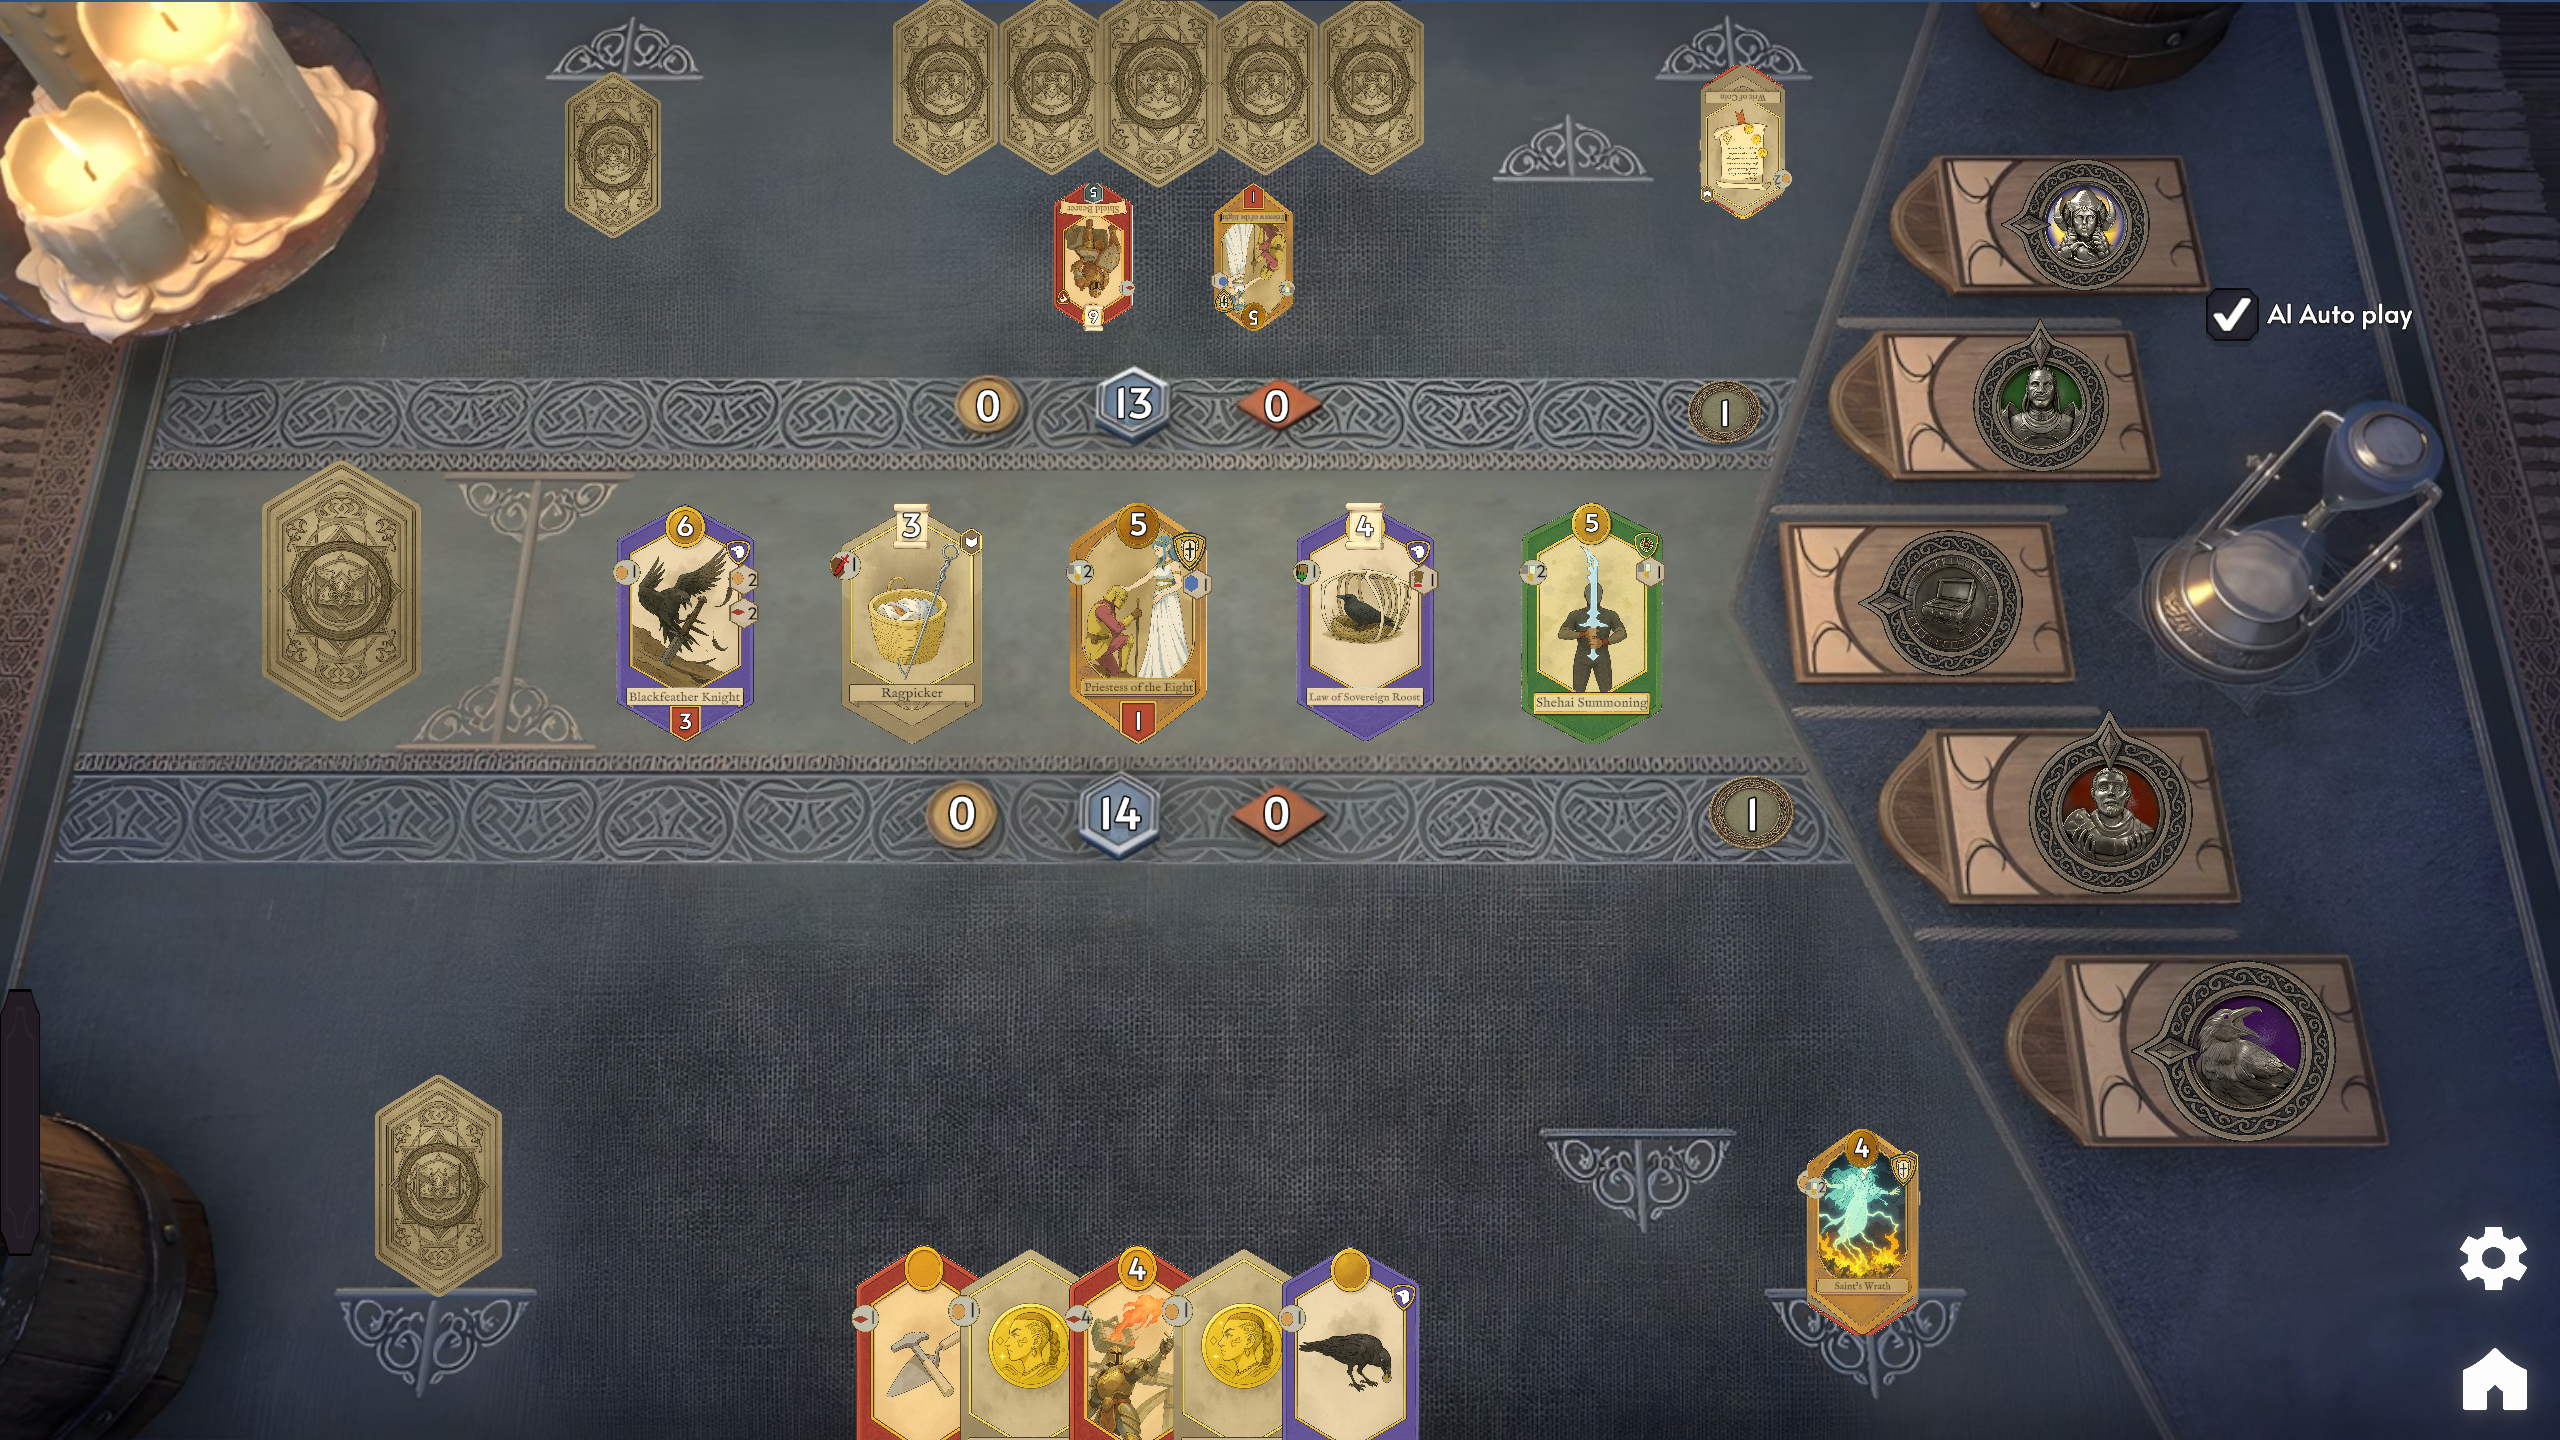
\includegraphics[width=1.0\textwidth]{img/GameView.png}
	\caption{Tablero de juego de SoT. \cite{ematerasu_scriptsoftribute-gui-20_2025}}
	\label{fig:game_view}
\end{figure}

El cliente gráfico también cuenta con pantallas específicas para las acciones especiales, en la figura \ref{fig:choice_panel} se muestra un ejemplo del panel de elección de descarte de cartas.

\begin{figure}[H]
	\centering
	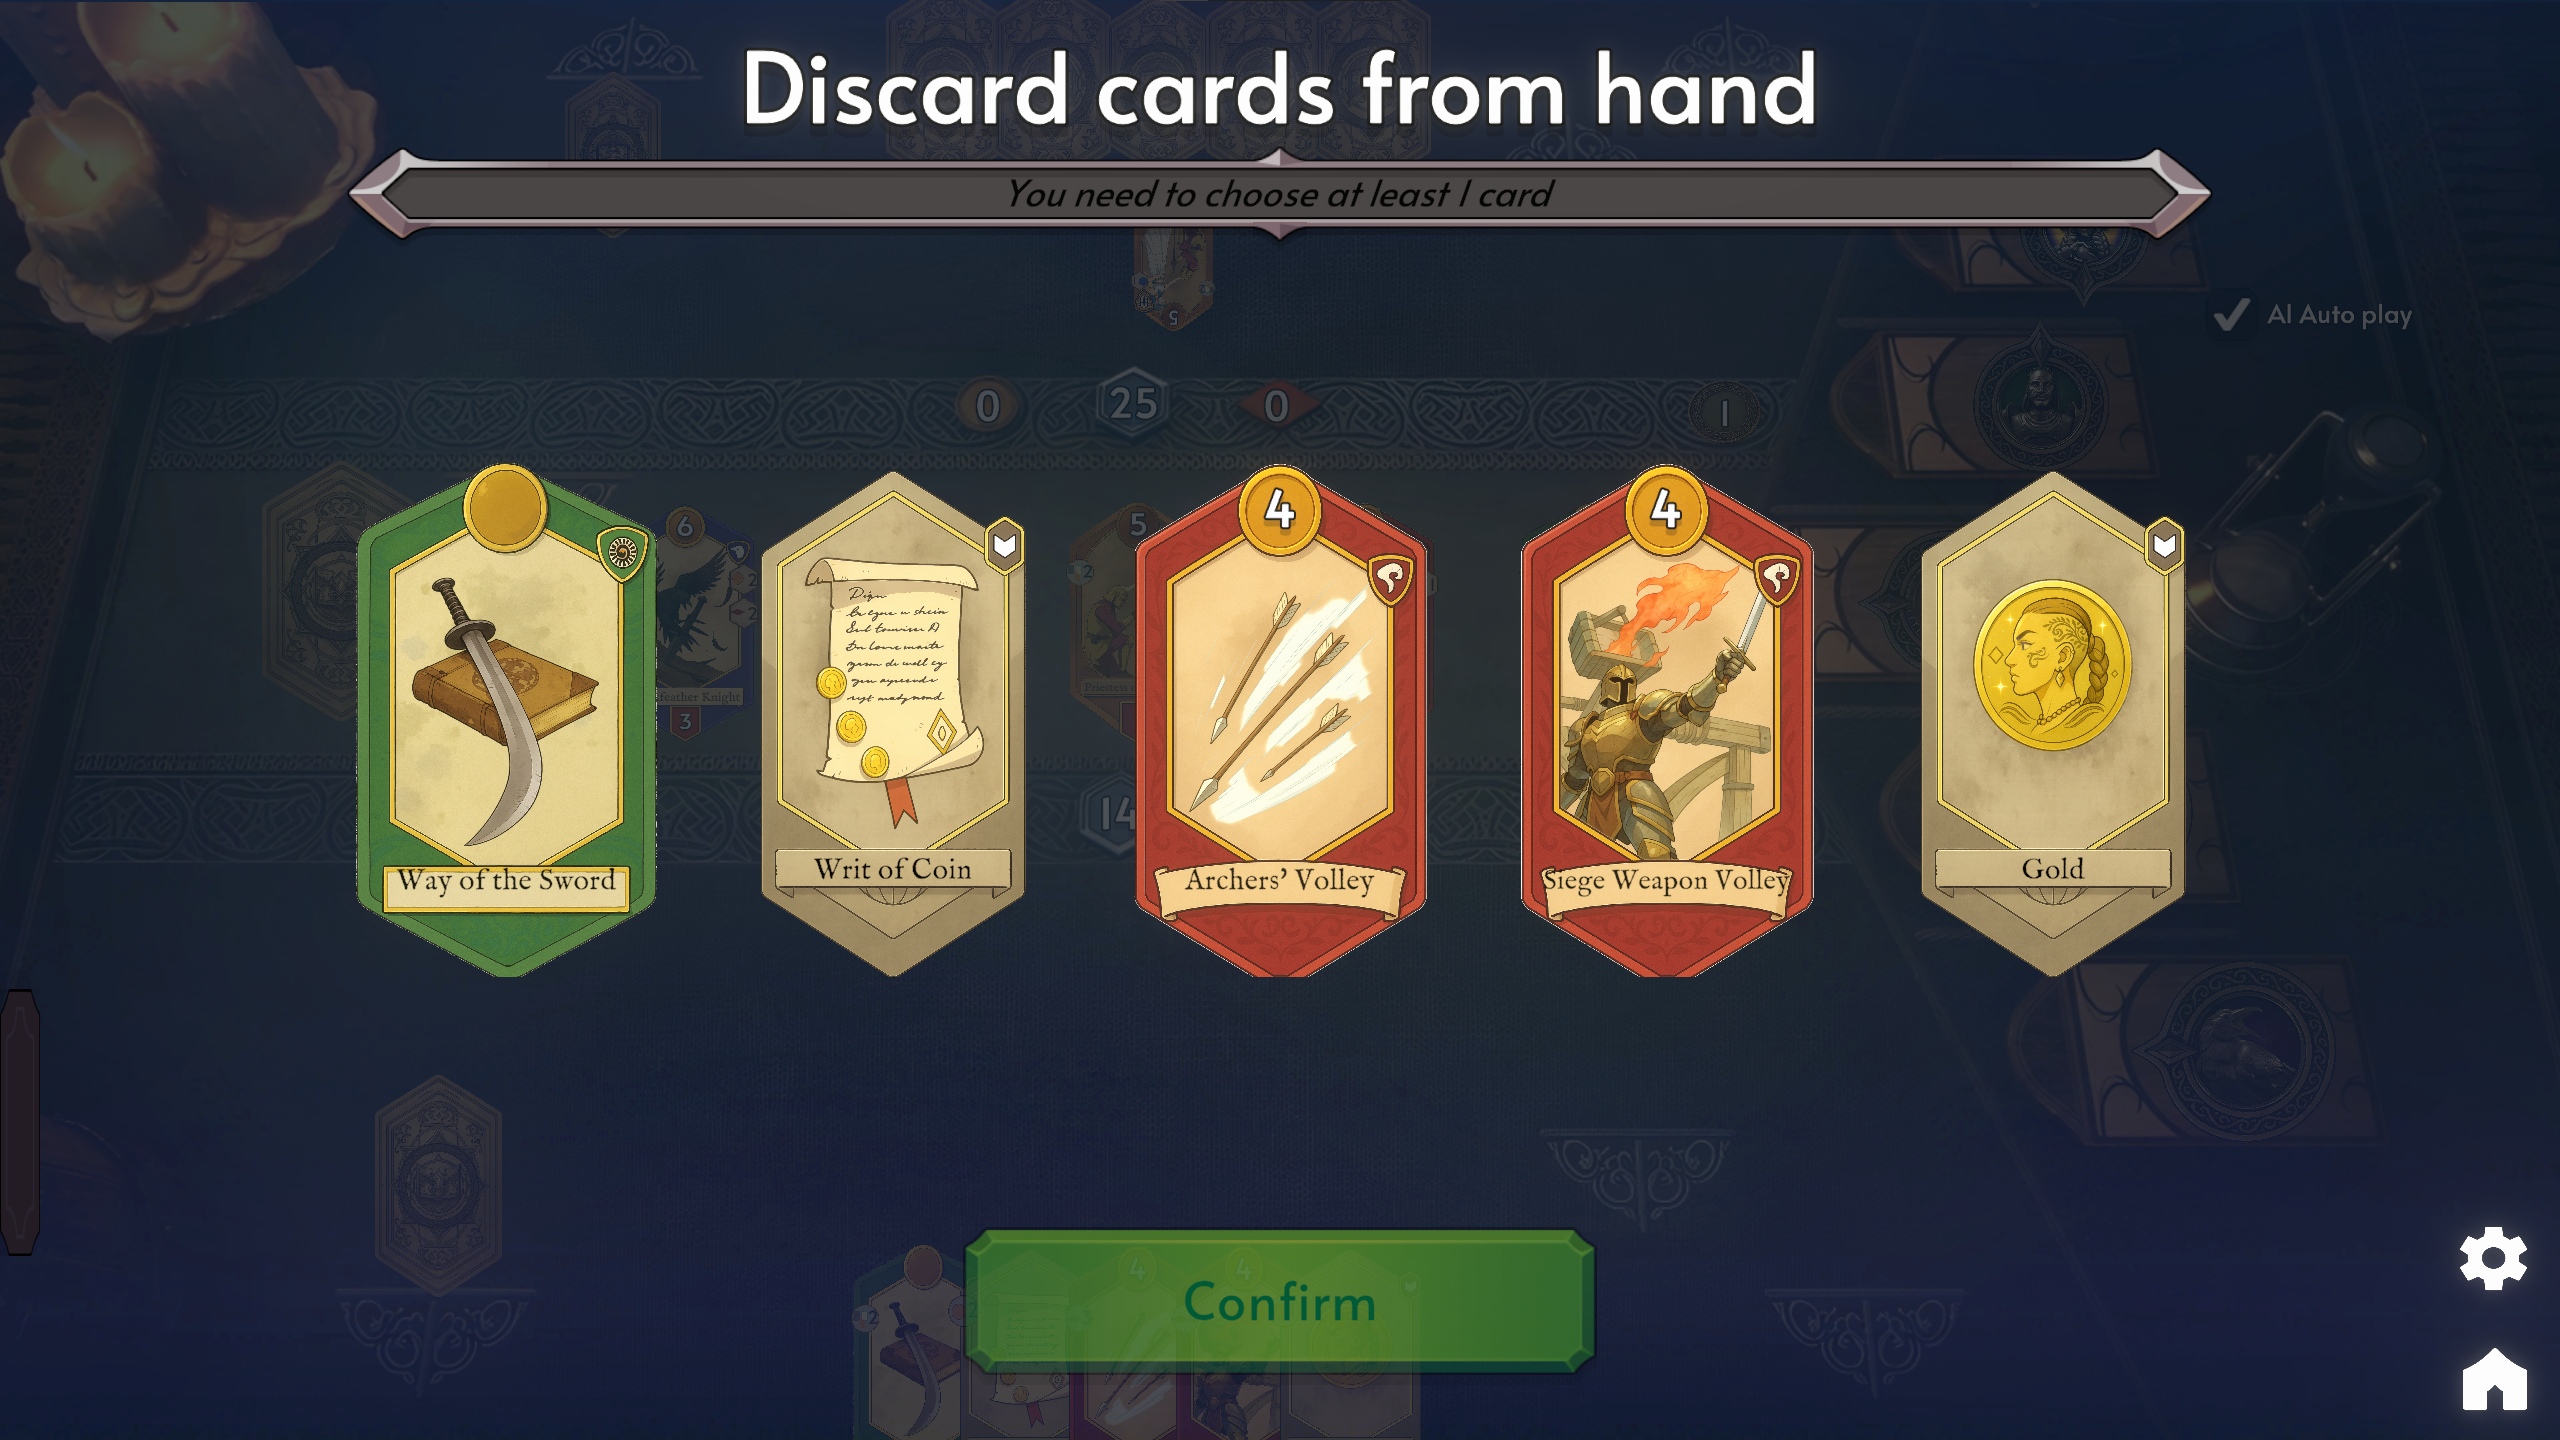
\includegraphics[width=1.0\textwidth]{img/ChoicePanel.png}
	\caption{Vista de elección de cartas en SoT. \cite{ematerasu_scriptsoftribute-gui-20_2025}}
	\label{fig:choice_panel}
\end{figure}

Finalmente, al concluir una partida, la interfaz presenta una pantalla de resumen como la de la figura \ref{fig:game_end}, donde se muestra el ganador y un historial completo de los movimientos realizados por ambos jugadores. Esto también se puede realizar con la versión de consola, pero la interfaz gráfica ofrece una visualización más intuitiva y accesible para el usuario.

\begin{figure}[H]
	\centering
	\includegraphics[width=1.0\textwidth]{img/GameEnd.png}
	\caption{Vista de final de partida con historial de movimientos en SoT. \cite{ematerasu_scriptsoftribute-gui-20_2025}}
	\label{fig:game_end}
\end{figure}

\subsection{Arquitectura del entorno} \label{sec:arquitectura_entorno}

El núcleo del motor de simulación, \textit{Scripts of Tribute-Core}, proporciona toda la lógica del juego y los puntos de entrada para el desarrollo de agentes. Para crear un nuevo bot, es necesario desarrollar una clase que herede de la clase abstracta ``AI.cs'' e implementar, como mínimo, dos métodos esenciales: ``SelectPatron'', que se encarga de la selección de patrones al inicio de la partida, y ``Play'', que se invoca repetidamente durante el turno del agente para que elija la siguiente acción a realizar. En cada llamada, el método ``Play'' recibe un objeto ``GameState'' que contiene una representación completa de toda la información visible en el juego, como las cartas en la mano, los agentes en el tablero o las cartas disponibles en la Taberna, permitiendo al bot tomar una decisión informada.

Si bien la interfaz gráfica es útil para la observación, la gran mayoría del trabajo de este proyecto se apoya en el ``GameRunner'', una aplicación de consola que forma parte del núcleo de SoT. Esta herramienta permite ejecutar un gran número de partidas entre dos bots especificados por línea de comandos, utilizando varios núcleos de la CPU para ejecutar tantas partidas simultáneas como se indique. Es precisamente este programa el invocado por el script de entrenamiento para cada una de las miles de evaluaciones que componen el proceso evolutivo.

Actualizaciones recientes en el motor han añadido la posibilidad de interactuar con agentes escritos en lenguajes externos mediante gRPC\footnote{gRPC es un sistema de código abierto desarrollado por Google para gestionar llamadas a procedimientos remotos (RPC) de alto rendimiento. Permite que un programa ejecute una función en otro proceso, incluso en una máquina diferente, como si fuera una llamada local \cite{google_grpc_2016}.}. Sin embargo, este proyecto inició su desarrollo antes de que esta funcionalidad estuviera disponible, por lo que el bot se tuvo que implementar en C\# y no en Python. Esto generó un problema de comunicación entre el script de entrenamiento y el bot, ya que el motor no permite la inyección de los pesos del bot directamente desde la línea de comandos. Para resolverlo, el script de ajuste de pesos (o ``entrenador'') establece los pesos del bot mediante variables de entorno del intérprete de comandos utilizado (ya sea bash o Powershell), que se leen a través de un método del bot antes de que comience la simulación. Esta dinámica permite que el algoritmo evolutivo en Python asigne pesos y evalúe el comportamiento del agente que opera dentro del entorno C\#.

Durante el continuo desarrollo del motor, Ematerasu et al. no solo han añadido nuevas opciones técnicas, sino también el nuevo contenido del juego. La edición de 2024 introdujo el mazo del patrón ``Rey Hechicero Orgnum'', mientras que la de 2025 añadió el de ``Santa Alessia''.

\section{La competición IEEE-CoG} \label{sec:competicion_ieee_cog}

Más allá de ser un simple motor de simulación, \textit{Scripts of Tribute} también se utiliza como plataforma para unas de las varias competiciones de inteligencia artificial celebradas anualmente en el congreso del \textit{IEEE Conference on Games} (CoG). El formato de la competición está diseñado para medir de forma robusta el rendimiento de los bots. Los agentes se enfrentan en un torneo de tipo \textit{Round-robin} (todos contra todos), donde el ganador se determina por el mayor porcentaje de victorias promedio tras un gran número de partidas espejo\footnote{En una ``partida espejo'', dos agentes A y B juegan una contra el otro dos veces, intercambiando la posición de jugador inicial en cada partida para asegurar la equidad.}. Las reglas imponen restricciones técnicas estrictas para los participantes, como un límite de tiempo de 10 segundos por turno y un uso de memoria que no debe exceder los 256 MB. Estas limitaciones obligan a los desarrolladores a buscar soluciones eficientes que equilibren la complejidad estratégica con el rendimiento computacional.

En la figura \ref{fig:competicion_ieee_cog_2024}, se muestran los resultados de la edición de 2024, donde el bot ya mencionado en la sección \ref{sec:mcts_cog} del capítulo anterior, gano por segundo a vez consecutiva. Los otros bots contaban con gran variedad de técnicas para su entrenamiento, desde MCTS hasta redes neuronales profundas e incluso aprendizaje por refuerzo.

\begin{figure}[H]
	\centering
	\includegraphics[width=1.0\textwidth]{img/ieee-cog-2024.png}
	\caption{Resultados de la competición IEEE-CoG 2024. \cite{ematerasu_scriptsoftribute-competitionsarchive_2024}}
	\label{fig:competicion_ieee_cog_2024}
\end{figure}

Este capítulo marca la conclusión del objetivo \textbf{OG1}, que consistía en analizar en profundidad las mecánicas del juego \textit{Tales of Tribute}, el entorno de desarrollo \textit{Scripts of Tribute} y adquirir las competencias necesarias en el lenguaje de programación C\#.
\chapter{Planificación del proyecto} \label{chap:planificacion}


\section{Recursos utilizados} \label{sec:recursos_utilizados}


\subsection{Recursos software} \label{sec:recursos_software}
% Lenguajes (C#, Python), Librerías (Inspyred, Pydantic, Pandas, Matplotlib, etc)
% VS Code
% Git
% LaTeX
% etc


\subsection{Recursos hardware} \label{sec:recursos_hardware}
% Especificaciones de mi PC y el de Pablo


\section{Metodología de desarrollo} \label{sec:metodologia_desarrollo}
% Metodología ágil mediante sprints (reuniones con Pablo)


\section{Distribución temporal y cronograma} \label{sec:cronograma}
% Diagrama de Gantt

\part{Metodología} \label{part:preparacion}
\chapter{Diseño del agente autónomo} \label{chap:software_bot}

En este capítulo se desglosa el diseño y la implementación del agente autónomo. El enfoque principal se centra en un sistema de toma de decisiones que evalúa cada acción posible mediante una función de puntuación ponderada, cuyos pesos son optimizados por el algoritmo evolutivo descrito en el siguiente capítulo. A continuación, se detallará la arquitectura de este sistema, la definición de los pesos que conforman su ``genoma'' y las lógicas específicas y heurísticas que complementan su comportamiento.

\section{Arquitectura de la toma de decisiones} \label{sec:arquitectura_toma_decisiones}

El comportamiento del agente se basa en una estrategia de decisión voraz con un horizonte de planificación de un solo paso. Cuando el bot debe realizar una acción, el motor del juego le proporciona una lista de todos los movimientos legalmente posibles. Para cada uno de estos movimientos, el bot realiza una simulación interna para averiguar como cambiaría el estado de la partida al aplicarlo. A este nuevo estado se le asigna una puntuación numérica a través de una función de evaluación heurística. Finalmente, el bot selecciona y ejecuta de forma determinista el movimiento que conduce al estado con la puntuación más alta, repitiendo este ciclo hasta que la acción elegida sea la de finalizar el turno. Esto contrasta con el enfoque de MCTS, pues en dicho algoritmo no se simula solo un movimiento, sino la partida entera en múltiples posibles ramificaciones. Una de las ventajas del enfoque voraz es su rapidez, en ningún momento se llegaría ni al límite de tiempo de 10 segundos por turno, ni al de memoria de 256 MB, lo que permite al bot tomar decisiones incluso en situaciones de alta presión temporal. Además, aunque el enfoque MCTS podría ofrecer una mejor exploración de las posibles jugadas, también es cierto que cuanto más se aleja del estado actual de la partida, más incertidumbre hay sobre el valor de las jugadas debido a la alta estocasticidad del juego y menos valor tendría la evaluación de un estado futuro lejano.

El punto más importante este sistema es la función de evaluación, ``ScoreMove'', que calcula la idoneidad de un estado del juego. Esta función es la que ejecuta la evaluación lineal ponderada, donde se calculan las diferencias entre el estado del juego antes y después de la jugada simulada a través de un conjunto de características. Cada una de estas características se multiplica por un peso específico, y la suma (o resta, en caso de gestionar datos relativos al contrincante) de todos estos componentes da como resultado la puntuación final de la acción.

La fórmula general que representa este cálculo se puede expresar según la ecuación \ref{eq:puntuacion_movimiento}:

\begin{equation}
\text{Puntuación}(m) = \sum_{i=1}^{n} w_i \cdot \Delta f_i(E_{t+1}, E_t) \label{eq:puntuacion_movimiento}
\end{equation}

Donde $\text{Puntuación}(m)$ es el valor asignado al movimiento $m$, $n$ es el número total de características evaluadas, $w_i$ es el peso asociado a la característica $i$, y $\Delta f_i$ es la función que calcula la diferencia de valor de dicha característica entre el estado resultante $E_{t+1}$ y el estado original $E_t$. Para garantizar que la comparación entre los diferentes movimientos sea reproducible, todas las simulaciones de acciones se realizan utilizando una semilla constante, lo que elimina la estocasticidad de ciertos eventos del juego, como el robo de cartas de la taberna. En el siguiente pseudocódigo se muestra el bucle de evaluación que sigue el bot para cada uno de los posibles movimientos:

\begin{algorithm}[H]
    \caption{Selección de la Mejor Acción en un Turno}
    \label{alg:get_best_move}
    \begin{algorithmic}[1]
        \State \Comment{Lógica interna del agente para elegir una acción en el estado de juego actual $S$.}
        \State \textbf{Entradas:} Estado del juego $S$, Lista de acciones posibles $A = \{a_1, ..., a_n\}$, Pesos $\vec{w}$.
        \State
        \State $\text{mejorAcción} \leftarrow \text{AcciónAleatoria}(A)$
        \State $\text{mejorPuntuación} \leftarrow -\infty$
        \State
        \State \textbf{para cada} acción $a_i \in A$ \textbf{hacer}
        \State \quad \textbf{si} $a_i$ es ``Pasar Turno'' \textbf{entonces}
        \State \qquad $\text{puntuación} \leftarrow -1$
        \State \quad \textbf{sino}
        \State \qquad $S_{t+1} \leftarrow \text{Simular}(S, a_i)$
        \State \qquad $\text{puntuación} \leftarrow \text{Evaluar}(S_{t+1}, S, \vec{w})$ \Comment{Usa la Ecuación \ref{eq:puntuacion_movimiento}.}
        \State \quad \textbf{fin si}
        \State
        \State \quad \textbf{si} $\text{puntuación} > \text{mejorPuntuación}$ \textbf{entonces}
        \State \qquad $\text{mejorPuntuación} \leftarrow \text{puntuación}$
        \State \qquad $\text{mejorAcción} \leftarrow a_i$
        \State \quad \textbf{fin si}
        \State \textbf{fin para}
        \State
        \State \textbf{devolver} $\text{mejorAcción}$
    \end{algorithmic}
\end{algorithm}

\section{Definición de los pesos} \label{sec:definicion_pesos}

El comportamiento estratégico del bot está enteramente definido por un conjunto de \textbf{20 pesos numéricos}. Este vector de valores representa el ``genoma'' de un individuo dentro del algoritmo evolutivo. Cada peso está asociado a una característica específica del juego, permitiendo al proceso de optimización ajustar con precisión la forma en que el bot valora cada aspecto de la partida. La Tabla \ref{tab:pesos_ebw} detalla cada uno de estos pesos y su función dentro de la evaluación.

La transferencia de estos pesos desde el entrenador al bot es un componente clave del sistema. Para evitar la sobrecarga de reescribir ficheros constantemente, el mecanismo principal se basa en el uso de variables de entorno. El script de Python convierte el genoma de un individuo (un array de 20 números) en una cadena de texto separada por comas. Esta cadena se asigna a una variable de entorno antes de lanzar el proceso del ``GameRunner''. Al iniciarse, el bot detecta estas variables, las lee, y utiliza sus valores para configurar la función de evaluación para esa partida en concreto.

	{\scriptsize
		\setlength{\tabcolsep}{4pt}
		\begin{longtable}{@{}l>{\tiny\raggedright\arraybackslash}p{2.2cm}p{0.65\textwidth}@{}}
			\caption{Descripción de los pesos del genoma del agente evolutivo.} \label{tab:pesos_ebw}                                                                                       \\

			\toprule
			\textbf{Categoría} & \textbf{Peso (Enum)} & \textbf{Descripción}                                                                                                                \\
			\midrule
			\endfirsthead

			\multicolumn{3}{c}{{\tablename\ \thetable{} -- Continuación}}                                                                                                                   \\
			\toprule
			\textbf{Categoría} & \textbf{Peso (Enum)} & \textbf{Descripción}                                                                                                                \\
			\midrule
			\endhead

			\midrule
			\multicolumn{3}{r}{{Continúa en la siguiente página}}                                                                                                                           \\
			\endfoot

			\bottomrule
			\endlastfoot

			\multirow{4}{*}{\begin{tabular}[c]{@{}l@{}}Agentes y\\ Combate\end{tabular}}
			                   & A\_HEALTH\_ REDUCED  & Penalización por el daño recibido por un agente propio, o bonificación por el daño infligido a un agente enemigo.                   \\
			                   & A\_KILLED            & Penalización si un agente propio es destruido, o bonificación equivalente si se destruye un agente enemigo.                         \\
			                   & A\_OWN\_AMOUNT       & Pondera la importancia de tener un mayor número de agentes en el tablero.                                                           \\
			                   & A\_ENEMY\_ AMOUNT    & Pondera la importancia de que el enemigo tenga un mayor número de agentes en el tablero.                                            \\
			\midrule
			\multirow{8}{*}{\begin{tabular}[c]{@{}l@{}}Recursos y\\ Cartas\end{tabular}}
			                   & CURSE\_REMOVED       & Bonificación por eliminar una carta de maldición del propio mazo.                                                                   \\
			                   & C\_TIER\_POOL        & Valor asignado a las cartas del mazo según una clasificación de tier predefinida.                                                   \\
			                   & C\_TIER\_TAVERN      & Penalización por dejar cartas de tier alto disponibles para el oponente en la taberna.                                              \\
			                   & C\_GOLD\_COST        & Valor asignado a las cartas en función de su coste en oro.                                                                          \\
			                   & C\_OWN\_COMBO        & Bonificación por tener varias cartas del mismo patrón en el mazo, aumentando el potencial de combo.                                 \\
			                   & C\_ENEMY\_COMBO      & Pondera el potencial de combo del mazo del oponente.                                                                                \\
			                   & COIN\_AMOUNT         & Pondera la diferencia de monedas generadas en un turno.                                                                             \\
			                   & POWER\_AMOUNT        & Pondera la diferencia de poder generado en un turno.                                                                                \\
			                   & PRESTIGE\_AMOUNT     & Pondera la diferencia de prestigio ganado o perdido.                                                                                \\
			                   & H\_DRAFT             & Peso que se utiliza como multiplicador defensivo para valorar la acción de quitarle una carta útil al oponente (``hate drafting''). \\
			\midrule
			\multirow{5}{*}{\begin{tabular}[c]{@{}l@{}}Cartas\\ Específicas\end{tabular}}
			                   & T\_TITHE             & Valor asignado a la carta ``Tithe'', que permite una activación de patrón adicional.                                                \\
			                   & T\_BLACK\_ SACRAMENT & Valor asignado a ``Black Sacrament'', que permite destruir un agente enemigo.                                                       \\
			                   & T\_AMBUSH            & Valor asignado a ``Ambush'', que permite destruir hasta dos agentes enemigos.                                                       \\
			                   & T\_BLACKMAIL         & Valor asignado a ``Blackmail'', que proporciona poder o prestigio.                                                                  \\
			                   & T\_IMPRISONMENT      & Valor asignado a ``Imprisonment'', similar a ``Blackmail'' pero con mayor potencial.                                                \\
			\midrule
			\multirow{1}{*}{Patrones}
			                   & P\_AMOUNT            & Valor asignado a cualquier acción que cambie el favor de un patrón.                                                                 \\
		\end{longtable}
	}

\section{Lógicas específicas y heurísticas} \label{sec:logicas_especificas}

Para aquellos casos especiales en los que el bot puede no ser capaz de discernir la importancia de una jugada, como es el caso de la aparición en la taberna de ciertas cartas importantes, se implementaron una serie de lógicas específicas y heurísticas codificadas manualmente pero con su propio peso asignado.

El ejemplo más representativo se encuentra en la función ``CalculateTavernScore''. Esta función no evalúa el valor de adquirir una carta de la taberna para uno mismo, sino que calcula el valor estratégico de eliminarla de la taberna para que el oponente no pueda adquirirla. Esta técnica, popularmente denominada como \textbf{hate drafting}, se implementó tras ver a algunos jugadores explicar sus movimientos mientras jugaban. En los vídeos se observaba que a veces preferían quitarle una carta al oponente aunque no les fuera útil a ellos mismos, pues que el rival la utilizase sería peor que los recursos gastados en comprar la carta. Este cálculo es puramente heurístico y depende del estado actual de la partida. Por ejemplo, para la carta ``Tithe'', que permite una activación de patrón adicional, el bot la valora más positivamente de forma defensiva (es decir, quitarla para que el oponente no la compre) si el oponente está cerca de alcanzar la victoria por prestigio, ya que un turno con dos acciones de patrón podría ser decisivo para él. De forma similar, se evalúan otras cartas clave como ``Ambush'', cuyo valor aumenta exponencialmente cuantos más agentes tenga el oponente en el tablero.

Además de esta lógica centrada en la taberna, existen otras heurísticas integradas en la evaluación. En ``CalculateScoreAgents'', por ejemplo, se diferencia entre simplemente dañar a un agente y destruirlo por completo, asignando una penalización mucho mayor a esto último. Asimismo, en la función ``ComputeCardPoolValue'' se aplica una lógica especial para las cartas de \textbf{maldición}: tenerlas en el propio mazo es negativo, pero conseguir que el oponente adquiera una es positivo. Esta combinación de una función de evaluación general y optimizable con heurísticas específicas para casos concretos intenta unificar el conocimiento del jugador con la potencia bruta de la optimización evolutiva. El sistema evolutivo se encarga de ajustar el comportamiento general, mientras que el conocimiento codificado en las heurísticas garantiza que el bot actúe de forma decisiva en momentos clave de la partida.

El desarrollo del bot marca el cumplimiento del \textbf{OG2}, que establece el diseño e implementación un agente inteligente en C\# para \textit{Scripts of Tribute}, cuya toma de decisiones se base en una evaluación heurística del estado del juego mediante una función de fitness ponderada, incorporando conocimiento específico del dominio.
\chapter{Sistema de entrenamiento evolutivo}
% La parte en Python

\section{Arquitectura general del entrenador}
% Visión general del sistema. Script en Python que usa Inspyred para orquestar un algoritmo evolutivo
% Encontrar el conjunto de pesos óptimo para el bot
% Diagrama de flujo

\section{Comunicación entrenador-imulador}
% Los subprocesos y las variables de entorno
% os.environ para pasar los pesos de un individuo al bot en C#

\section{El algoritmo evolutivo con Inspyred}
% Justificar la elección de Inspyred
% Describir los componentes de un EA: individuos, población, generación inicial, operadores de variación, evaluación del fitness, selección, etc
% Explicar los valores por defecto de Inspyred

\section{Paralelización del algoritmo}
% Uso de multiprocessing para el diccionario y concurrent.futures para el evaluador

\section{Mecanismos de evaluación del fitness}

\subsection{Modo fijo: evaluación contra oponentes estáticos}
% El individuo juega contra un conjunto predefinido de bots. El fitness es el número de victorias
% inspyred.ec.evaluators.parallel_evaluation_mp
\subsection{Modo coevolución: competición interna}
% Los individuos (padres e hijos) compiten entre sí en un torneo round robin. El fitness es el número de victorias
% evaluate_coevolution_orchestrator
\subsection{Modo híbrido: combinando estrategias}
% Sistema de entrenamiento por segmentos hybrid_schedule_str
% Gestión de cambios de modo
\section{El salón de la fama}
% Mantener un diccionario de oponentes de élite (catastrophic forgetting)

\part{Experimentación y conclusiones} \label{part:resultados}
\chapter{Diseño experimental} \label{chap:experimentacion}
% Como se prueban los bots

\todo{Probar diferentes combinaciones en el modo hibrido.}
\todo{Hablar sobre los individuos generalistas (todos los pesos parecidos) y especialistas (0-1 en los pesos) en los mejores pesos.}
\todo{Ver la diferencia entre usar el hall of fame y no usarlo ya que no debería añadir info de una train run a otra. Mirar en la literatura que es exactamente hall of fame.}
\todo{Para comparar los modos de entrenamiento, intentar que todos los algoritmos se ejecuten durante la misma cantidad de tiempo (aunque tengan tamaños de poblaciones diferentes).}
\todo{Lanzar sin el hall of fame para evitar las diferencias entre runs.}

\section{Configuración de los experimentos} \label{sec:configuracion_experimentos}
% Entrenamiento en modo Coevolución
% Entrenamiento en modo Híbrido con varias organizaciones
% Parámetros utilizados de configuración


\section{Métricas de evaluación} \label{sec:metricas_evaluacion}
% Evolución del fitness (máximo, medio, mínimo) a lo largo de las generaciones
% Convergencia y distribución de los pesos de la población
% Rendimiento del "campeón" de cada `train_run` en el benchmark final y contra otros bots fuera del entrenador
\chapter{Resultados y discusión} \label{chap:resultados}
% Interpretar los resultados de cómo y por qué
% - ¿Por qué el modo híbrido funciona mejor que los otros?
% - La tendencia de los pesos a irse a 0 o 1
% - Limitaciones del enfoque: bot sin memoria ni planificación, etc

\section{A nivel de población} \label{sec:a_nivel_de_poblacion}


\subsection{Evolución del fitness} \label{sec:evolucion_fitness_poblacion}


\subsection{Pesos medios} \label{sec:pesos_medios_poblacion}


\subsection{Pesos a lo largo de las generaciones} \label{sec:pesos_a_lo_largo_generaciones_poblacion}


\subsection{Variación de los pesos finales} \label{sec:variacion_pesos_finales_poblacion}


\section{A nivel de líderes} \label{sec:a_nivel_de_lideres}


\subsection{Evolución del fitness} \label{sec:evolucion_fitness_lideres}


\subsection{Pesos medios} \label{sec:pesos_medios_lideres}


\subsection{Pesos a lo largo de las generaciones} \label{sec:pesos_a_lo_largo_generaciones_lideres}


\subsection{Variación de los pesos finales} \label{sec:variacion_pesos_finales_lideres}





% https://en.wikipedia.org/wiki/AlphaStar_(software)
% https://www.bbc.com/news/technology-50212841
% Unlike AlphaZero, AlphaStar initially learns to imitate the moves of the best players in its database of human vs. human games; this step is necessary to solve what DeepMind's Dave Silver calls "the exploration problem": discovering new strategies would otherwise be like finding a "needle in a haystack". Agents then play each other and deploy deep reinforcement learning. These main agents also learn by playing against suboptimal "exploiter agents" whose purpose is to expose weaknesses in the main agents.
\chapter{Conclusiones} \label{chap:conclusiones}


\section{Objetivos alcanzados} \label{sec:objetivos_alcanzados}
% Resumen los hallazgos
% Explicar punto por punto qué objetivos se han cumplido


\section{Líneas de trabajo futuro} \label{sec:trabajo_futuro}
% Probar operadores de mutación y cruce más sofisticados
% Expandir el conjunto de oponentes fijos o dinámicos
% Implementar estrategias de coevolución más complejas

% Material de referencia
\backmatter

% % Bibliografía
\cleardoublepage
\bibliographystyle{plainurl}
\bibliography{bibliografia}

% \appendix
% \input{apendices/codigo}

\end{document}